%!TEX root = Manuscript.tex

\chapter{Algorithmic and industrial context}
\label{chap:context}
\minitoc

\section{Industrial context}
\subsection{What is 5G ?}



Telecoms networks must manage more and more users while providing them a better bandwidth, latency and reliability. Nowadays, 4G is the standard deployed in most of the territory, and a new technology is starting to be deployed: 5G. The term 5G covers a set of functional specifications. The organism that sets these specifications is the ITU (International Telecommunication Union). For several years, the ITU, more precisely the ITU-R (radiocommunication component of the ITU) has been working to determine the functional aspects that 5G must satisfy. Figure~\ref{fig:5gperf} from~\cite{dahlman20185g} illustrates some of those functional aspects, that ITU-R has formally referenced in IMT-2020 (the requirments of 4G are referenced in IMT-advanced): a bitrate up to 20Gbps ($\times 20 $compared to 4G), low end to end latencies down to 1ms ($10$ times lower than in 4G, we are focusing on this aspect in this thesis).
Also, 5G aims to offer an higher connection density (up to 1 million device$/km^2$), with an higher traffic capacity (from $0,1 Mbit/s/m^2$ in 4G to $10 Mbit/s/m^2$ in 5G) due to a larger uses of the spectrum. Others aspects as a better energy efficiency ($100$ times better in 5G than in 4G) or a better mobility are ensured. 

  \begin{figure}[h]
      \begin{center}
      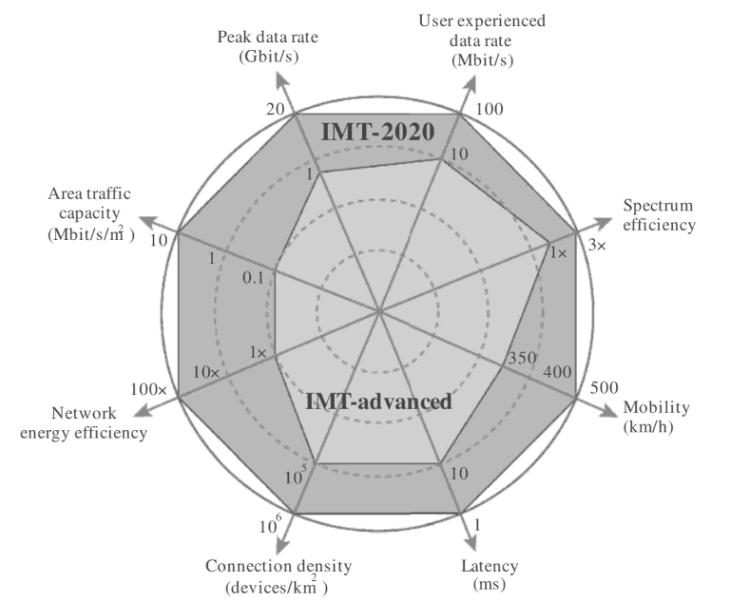
\includegraphics[width=1\textwidth]{Chapitre1/5Grequirements}
      \end{center}
      \caption{5G performances required by ITU-R}\label{fig:5gperf}
      \end{figure}

All these aspects lead us to various application cases. Figure~\ref{fig:usecases} taken from~\cite{5GACIA} establishes a non-exhaustive list of them, according to their different technical constraints. Indeed, low latency is required for applications like motion control that work in real time since one of the goals of 5G is to obtain dynamic programmable networks, for greater flexibility of use.
On the other hand, an higher bandwidth is usefull for applications like video streaming, augmented reality of ensuring the connectivity of a large number of terminals. By relaxing latency and broadband constraints, it is possible to expand further the number of devices (up to 1 million) for applications like sensors networks.

  \begin{figure}[h] 
      \begin{center}
      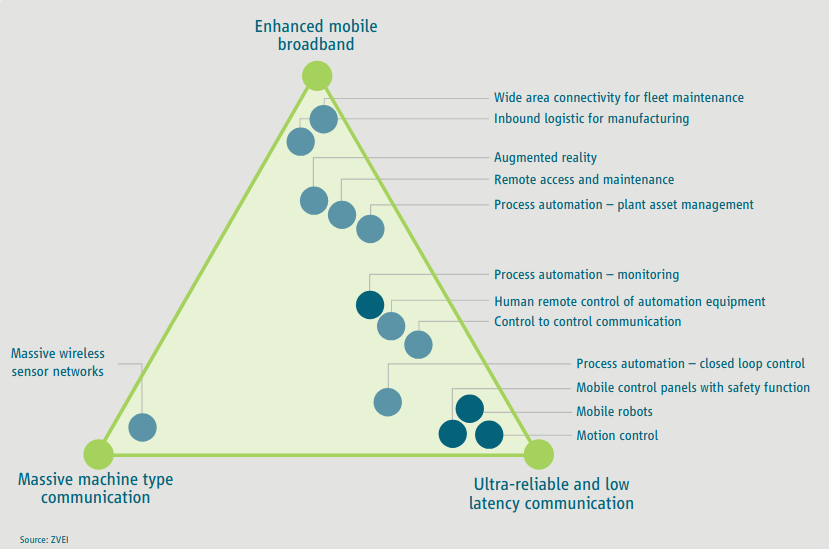
\includegraphics[width=1\textwidth]{Chapitre1/usecases.png}
      \end{center}
      \caption{Some examples of use cases for 5G}\label{fig:usecases}
      \end{figure}
          
\subsection{URLLC}


To meet these 5G functional specifications, the network equipments must follow some technical standards. 3GPP (3rd Generation Partnership Project) is an union between several standard organization which sets the technical specifications of 5G. 3GPP frequently publishes releases, that regroup new specifications. The first release focused on 5G was release 15, released in 2018 \cite{RELEASENOKIA}.  

  \begin{figure}[h]
      \begin{center}
      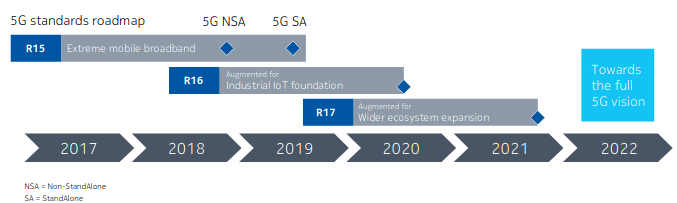
\includegraphics[width=1\textwidth]{Chapitre1/release.png}
      \end{center}
      \caption{3GPP releases 15, 16 and 17 calendar}\label{fig:release}
      \end{figure}
  
Release 15 focused on increasing throughput and interworking between 4G and 5G, and introduced the notion of URLLC (Ultra-Reliable Low-Latency Communication). Releases 16 an 17 have extended the notion of URLLC. The notion of URLLC consists in ensuring a low packet loss and a low latency communication. Indeed, several use cases (smart factories, control operations, \dots) needs some highly reliable communications in which the latency must be bounded. Most of the current network does not ensure a bounded latency for all packets. This is why we talk about statistical multiplexing; the latency of a given network is, most of the time good, but the technology does not ensure a maximal latency for $100\%$ of the packets.  In this thesis, we focus on the low latency aspect of our communication. More precisely, URLLC aims to ensure a good end to end latency. To achieve such a goal, each component of the communication must meet the constraints, the radio communications, and the core network. This thesis focus on the core networks. 

\subsection{5G Radio Access Network}
To understand on which part of the network this thesis focuses on, we might describe how does a radio access network works.

 \begin{figure}[h]
      \begin{center}
      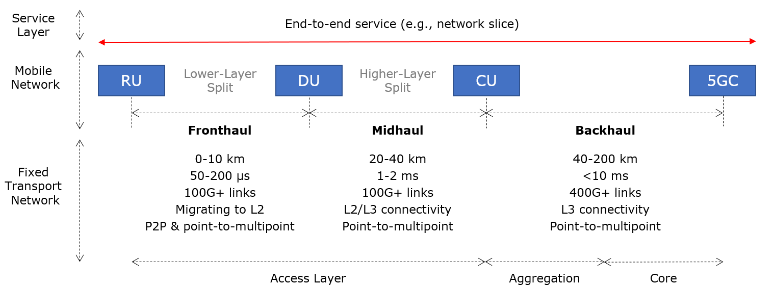
\includegraphics[width=1\textwidth]{Chapitre1/5gran.png}
      \end{center}
      \caption{5G Radio acess network}\label{fig:5gran}
      \end{figure}

\subsubsection{Cloud RAN}
Current mobile network (aka cellular network) architecture consists in a distributed radio access networks: the mobile terminals connect to base stations (BTS for Base Transceiver Station as a generic name, eNB for evolved Node B in 3GPP LTE “4G” standard) that encompasses all the sub-systems needed to realize mobile communication~\cite{bouguen2012lte}. It mainly comprises the radio part, that furnishes the connection between the mobile terminal and the BTS, and the network part that provides control and management functions like mobility support (the main functionality being the support of handover from one BTS to another, i.e. the ability to pursue a communication when moving from range of an antenna to another). The evolutions proposed in next generations aim at evolving toward centralized radio network architectures (C-RAN, for Cloud Radio Access Network) to reduce consumption costs and power at the base stations~\cite{mobile2011c}. These C-RAN architectures include simplified base stations on the field. Depending on the architecture choice  
, it can be restricted to the radio part and the digital to analog conversion only. This can be identified by different names depending on the reference documents, including RU for Remote Unit or Remote Radio Heads (RRH). The later will be used the rest of the document. The other component of the C-RAN is composed of the processing units (baseband unit: BBU – used in this document – or FU for Frontend Unit) located in the cloud. By cloud we define in this document the capability of instantiating executable programs in data centers that are transparently connected to the systems requiring the results of the program execution. The execution may be indifferently performed on virtualized machines, or bare metal one, or any other combinations. The network between RRH and BBU is called “Fronthaul Network”, or “Fronthaul” for short. Figure~\ref{fig:fronthaul} illustrates an example of fronthaul in which several BBU are gathered in a same datacenter. 

  \begin{figure}[h]
      \begin{center}
      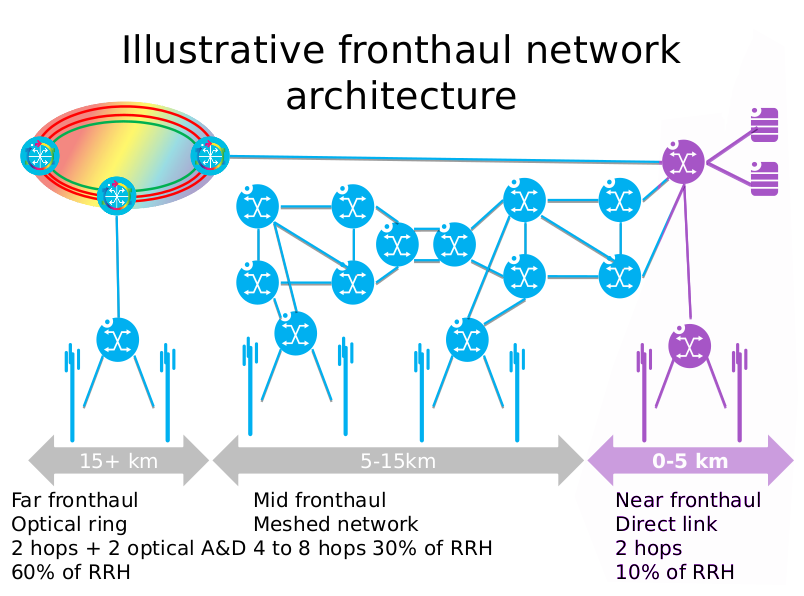
\includegraphics[width=1\textwidth]{Chapitre1/fronthaul.png}
      \end{center}
      \caption{An example of fronthaul network for Clound RAN}\label{fig:fronthaul}
      \end{figure}
      
      Figure~\ref{fig:CRANsplit} illustrates the two different ways proposed to split the BTS. In the first one, called ``Full centralization'' the RRH integrates only the radio functions, while in the second one, called ``partial centralization'', the RRH keeps the baseband processing function. In the last case, the term BBU is not apropriate anymore but is still used, in order to simplify the comprehension.
      
   \begin{figure}[h]
      \begin{center}
      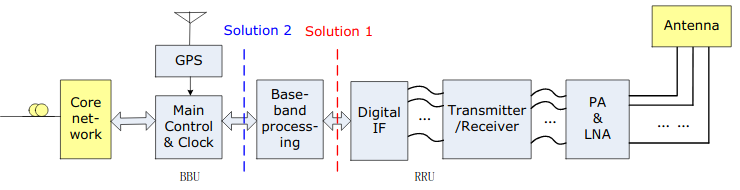
\includegraphics[width=1\textwidth]{Chapitre1/CRANsplit.png}
      \end{center}
      \caption{The two different split for Cloud-RAN}\label{fig:CRANsplit}
      \end{figure}
      \begin{figure}[h]
      \begin{center}
      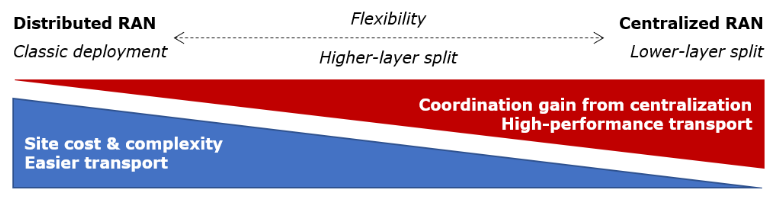
\includegraphics[width=1\textwidth]{Chapitre1/flexibility.png}
      \end{center}
      \caption{The more centralized is the RAN, the hardest is the transport and the lowest is the cost of coordination for the antennas}\label{fig:flexibility}
      \end{figure}
       
This type of architecture faces the challenge of mastering the latency in the transfer process between the RRHs on the field and BBUs in the cloud. Low latency is already critical for the deployment of C-RAN approach in LTE “4G” networks. The standard requires hard time constraints for functions like HARQ (Hybrid Automatic Repeat reQuest) that needs to be processed in less than $3ms$ \cite{bouguen2012lte}. Considering processing time into the BBU, the time budget over the network can be as low as $400\mu s$ for a round trip. One specificity in this C-RAN context is not only the latency constraint, but also the periodicity of the data transfer between RRH and BBU (this HARQ constraint must be enforced for each frame emitted every millisecond). Looking beyond current mobile network generation, one must have in mind that ongoing 5G standards will require to reach end-to-end expected latency as low as $1ms$ (depending on targeted services)~\cite{boccardi2014five}. New scheduling and new technologies have to be considered to guarantee delay constrained periodic data transfers. 


\subsection{Technical solution for low latency}


The expressed constraints expressed for C-RAN architecture and 5G standard are hardly met in current networks. In IP or even Ethernet networks, the traffic usually suffers of delay due to buffering. The amazing success of the packet based networks for the last 40 years relies on the statistical multiplexing: the packets are sent when they are ready and are buffered in intermediate nodes (routers for IP networks, switches for Ethernet networks) when contention arises \cite{venkatramani1994supporting}. A contention means that one resource (node out interface) is needed at the same time for transmission of several packets. In this case, the supplementary packets are stored in a buffer until the resources become available. This allows an easy deployment and management of a network, leading to a delivery of the packet with few loss (under conditions that buffers are big enough) but at the price of uncertainty on the delivery time. This uncontrolled and non predictable delay prevents to offer low latency and no jitter in the current network. Statistically managed QoS do not allow contention avoidance, then they can not provide null jitter \cite{khaunte2003technique}. If they can be used to prioritize some packets over the others (e.g. Express Forwarding against Best Effort), they fail to ensure delivery of a given packet in a given time delay when several packets compete for the same resource. 
The best current solution is to rely on an almost full optical approach, where each end-points (RRH on one side, BBU on the other side) are connected through direct fiber or full optical switches \cite{leclerc2016transmission}\cite{leclerc2016signaling}. This architecture is very expensive and hardly scales in the case of a mobile network. As illustrative purpose, a single (one operator) mobile network in France is composed of about $10,000$ base stations. This number will increase by a factor of $2$ to $20$ with the emergence of “small cells” that allow increasing base station density and to reach higher throughput \cite{leclerc2016transmission}\cite{leclerc2016signaling}. It is then needed to find a solution to offer low latency over commoditized packet based networks. 

Although 3GPP standards for 5G are not yet completely frozen, the core networks should use ethernet technology. Time Sensitive Networking (TSN) is a task group of IEEE that develop some standards in ethernet. The two standards we focus here are 802.1Qbu and 802.1Qbv \cite{ieee802}  
  
802.1Qbu allows frame preemption, that is, a node of the network is able to stop the transmission of a frame to send another frame. This brings us to a management of networks in which some flow can be considered as more critical than others. 

\todo{si on garde, schema + explications} 

802.1Qbv allows the nodes to manage different flows by a gate mechanism. Knowing the flows travelling over a node of the network, it is possible to schedule on an output port the time at which each flow must be sent by the node in order to prioritize the most critical flows. The scheduler sends a  GCL (gate control list) to the node. To one gate is associated one or several flows, and the nodes open or close the gates following the GCL.

Figure~\ref{fig:tsnqbv} found in \cite{durr2016no} shows the mechanism of a switch with the 802.1Qbv technology. Considering a given period ($T_{cycle}$ in the figure), the switch select at each times ($T_1 , T_2 , \ldots$ the queues that must be open to transmit packets. In figure 6, at time $T_1$, all gates exept the one for scheduled traffic are open, at time $T_2$, all gates are closed and at time $T_3$ only the gate for scheduled traffic is open.
  \begin{figure}[h]
      \begin{center}
      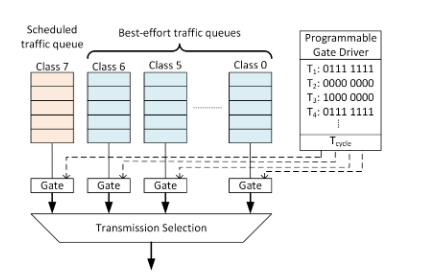
\includegraphics[width=0.8\textwidth]{Chapitre1/tsnqbv.png}
      \end{center}
      \caption{IEEE 802.1Qbv mechanism}\label{fig:tsnqbv}
      \end{figure}
      
   
\section{Algorithmic related works}

  We show in this article that statistical multiplexing, even in a fronthaul network with a small load, does not comply with the latency requirements of C-RAN. Therefore, current solutions~\cite{pizzinat2015things,tayq2017real}  use dedicated circuits for the fronthaul. Each end-point (RRH on one side, BBU on the other side) is connected through direct fiber or full optical switches. This architecture is very expensive and hardly scales in the case of a mobile network composed of about $10,000$ base stations. The deterministic approach we propose has gained some traction recently: Deterministic Networking is under standardization in IEEE 802.1 TSN group~\cite{finn-detnet-architecture-08}, as well at IETF DetNet working group~\cite{ieee802}. Several patents on concepts and mechanisms for DetNet have been already published, see for example~\cite{howe2005time,leclerc2016transmission}. 
     
The algorithmic problem we focus on may look like wormhole problems~\cite{cole1996benefit}, but we want to minimize the time lost in buffers and not just to avoid deadlocks. Several graph colorings have been introduced to model similar problems such as the allocation of frequencies~\cite{borndorfer1998frequency}, bandwidths~\cite{erlebach2001complexity} or routes~\cite{cole1996benefit} in a network. Unfortunately, they do not take into account the periodicity of the scheduling and the associated problems are already $\NP$-complete. The only coloring with periodicity is the circular coloring~\cite{zhou2013multiple} but it is not expressive enough to capture our problem. 
The problem \pall on a star routed network is very close to a two flow-shop scheduling problem~\cite{yu2004minimizing} with the additional constraint of periodicity. To our knowledge, all studied periodic scheduling problems are different from \pall that we consider in this article. 
Either the aim is to minimize the number of processors on which the periodic tasks are scheduled~\cite{korst1991periodic,hanen1993cyclic} while our problem correspond to a single processor and a constraint similar to makespan minimization. Or, in cyclic scheduling~\cite{levner2010complexity}, the aim is to minimize the period of a scheduling to maximize the throughput, while our period is fixed. 

The train timetabling problem~\cite{lusby2011railway} and its restriction, the periodic event scheduling problem~\cite{serafini1989mathematical} are generalizations of our problem. Indeed, they take the period as input and can express the fact that two trains (like two messages) should not cross. However, they are much more general: the trains can vary in size, speed, the network can be more complex than a single track and there are precedence constraints. Hence, the numerous variants of train scheduling problems are very hard to solve (and always $\NP$-hard). Thus, some delay is allowed to make the problems solvable and most of the research done~\cite{lusby2011railway} is devising practical algorithms using branch and bound, mixed integer programming, genetic algorithms\dots  In the same spirit, complex scheduling problems for time sensitive networks have also been practically solved, using mixed integer programming~\cite{nayak2017incremental,steiner2018traffic} or an SMT solver~\cite{dos2019tsnsched}.



Expliquer la litérature, et ce qui diffère de notre pb à nous